\chapauth{murdered by owls}
\chapter[The One Act Remaining]{The One Act Remaining To Me In This World}





I'm not sure how it is possible for me to sit here, outwardly
so calm, while a tornado is whipping around inside my brain,
flinging emotions about like bits of debris left over from an
explosion in a sex shop. The definition of surreal: digging dildo
shards out of your ears{\ldots} if only metaphorically.



I glance out the window of the break room of the factory where I
work, and notice that the moon is full, gravid with cold
purple-white light. Why does it seem to be calling me? I want to
understand what it is trying to tell me. I know it's telling
me something, if only I could hear it through the endless,
soundless muttering of a million dying souls. They're everywhere.
Their sighs fill my head like a swarm of crocheted bees.



My coffee is very hot, and tastes of metal, or perhaps the tears of
molested children. I'm not sure why that comes to mind. How
would I know what molested child tears taste like? A trivial
mystery to which I am unlikely ever to find an answer{\ldots}



There is a part of me, deep inside, that is like a tiger with
foot-long blades for claws, and it wants to attack and rip and
destroy this violent feeling of whirligig that raves and rages and
rapes the rest of my brain like a lunatic conquistador. But the
tiger cannot fight an opponent so vague and ephemeral. It's
like trying to grapple with a fart, or wage war against a cloud of
gnats armed only with a Beretta or a bag of tulips.



A solemn fog has grown out of the river just to the north of us,
and it is as though someone has thrown a gray blanket across the
fields surrounding the factory. The moon looks down on all this,
benign, but also wild and terrible, the face of a pagan goddess
with a cold and clear eye. This is somehow comforting.



Two of my fellow night shift machine operators walk in the room,
get their coffee and candy bars, and sit down at the other side of
the room, not speaking a word. We ignore each other testily. The
silence between us is a sacred bond, unrelenting, immutable. It is
more than just mute testimony to our deep and abiding wariness, it
is a black and shapeless ocean, seeming to drown the words we do
not speak.



It is all right; I have grown indifferent.



As I pick up the sports page from the table, I feel a sudden surge
of terror, coming from nowhere and everywhere, as if I had been
shaving in front of the bathroom mirror and seen a reflection of
the tiger streaking towards the back of my neck with deadly, fluid
speed, claws outstretched to rend and destroy.



Outside, I show nothing.



I sip my coffee.



My cock is hard as steel.



Ten minutes later, I am once again at the controls of my machine.
It vomits polyurethane airmail envelopes in an endless stream. The
stink of burning hot melt has settled into my clothing, and can be
sensed faintly anywhere I go, like the ghost of cheap aftershave on
a shirt the day after a date. Here, in the factory, the odor is
strong and almost palpable, with a kind of chewy, yellow
resonance.



My bagger stands at the far end of the monolithic, hissing metal
apparition and collects the envelopes as they are expectorated by
the machine onto a small table. He executes a kind of dance, the
steps repeating every thirty seconds or so. He watches the counter
over the cutter bar, and when it reaches 100, he snatches the pile
out from under the next envelope with greedy, clutching fingers and
slams it into the cardboard flat he has prepared. He folds the top
over, slaps a strip of tape over the seam, and stamps the side with
the date and shift, all in one long, fluid movement. He bends and
twirls, deftly slipping the flat into a bigger box on a pallet.
Then he returns to the table at the end of the machine and prepares
another flat with economical, practiced motions, and places it
before him, ready to enshroud the next stack of the machine's
ejecta. Waiting the next few seconds for the next stack to be
ready, he waits completely motionless, head down, his hands spread
out before him on the table.



I watch him carefully out of the corner of my eye as I run my
machine, and I wonder if he knows he is dancing. Could his
insensate eyes, half-closed and empty, simply be looking within,
seeing himself on some shadowy stage upon which he turns and
leaps?



Actually, I think he's dead, and like a freshly decapitated
chicken, he just hasn't noticed it yet. He's dancing,
all right, but it's the same kind of dance a fresh corpse
executes at the end of a rope after dropping through the trap door.
The ballet of the damned.



When the sun comes up outside, near the end of the shift, it always
seems to me like the whole factory and the buildings and fields
that surround it have been cruising all night through another
dimension, like a spaceship that goes through some kind of time
warp and then reemerges, unharmed and unchanged, at the exact
moment from which it departed. Nothing has changed in the world of
our origin, nothing has changed in our isolated pocket of reality,
but we have gone somewhere and come back nonetheless.



I know that when I leave the factory and drive home in my car, I
will feel like an unknown astronaut quietly and without fanfare
returning home after spending years alone in my ship. I will listen
to the sound of no crowds cheering and watch as no tickertape falls
to celebrate my arrival as I drive through still-slumbering
streets.



I am home, but I am still isolated and alone.



When I walk out the front door, the fog is still there. It writhes
its way down the length of the river, enclosing and concealing it
entirely. I idly speculate that there could be some strange things
going on in there, and nobody would ever know.



Anything could be hiding down there.



There's nothing there, of course. It's just idle
speculation.



I throw a rock down there as I walk past, just to be sure.



Nothing happens. I stand for a moment, listening, and then laugh
nervously and walk on.



I can feel the moon up there, smiling at me, even though it has
disappeared behind the trees. That's one thing about the
moon; you can count on it being there, even if you can't see
it.



If you saw me now, a nondescript man calmly walking to his
nondescript car at the end of another day at his nondescript job,
you would never guess that I'm going insane.



The impending death of my rationality is overtaking me like the
approach of a black hole, and within days, hours{\ldots} minutes,
maybe, I'm going to cross the event horizon and succumb to
the raging storm of gravitation spinning like a top within that
infinite silken darkness.



But before the dissonance of that crazy awakening rea\-ches its
crescendo, I'm going to perform the one act remaining for me
in this world.



I'm going to wear a pair of Jessica Alba's
panties.



Then I can finally die. 
 



\begin{figure}[b]
  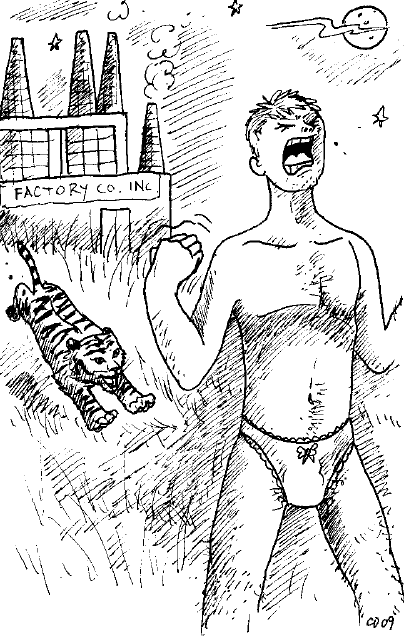
\includegraphics[width=\textwidth]{art/Part_of_Everything-Scream_in_Panties.png}
  \caption{Artwork by Part of Everything}
\end{figure}
